\section{Benchmark Programs}
\label{sec:benchmark}
 
We envisage GP 2 as a general-purpose language for graph problems, hence the reference interpreter should be tested on algorithms of varying complexity. This is different from the benchmarking reported in \cite{Varro-Schuerr-Varro05a} which focusses on a deterministic program with very limited complexity. In Section \ref{sec:performanceevaluation}, we evaluate the performance of our interpreter on a small set of benchmark programs. These include the programs for transitive closure and vertex colouring, and three more programs which we describe in this section.

\vspace{.5\baselineskip}
\noindent
\emph{Shortest distances.} The program in Figure \ref{fig:shortest-distances} expects an input graph $G$\/ containing a unique grey node $s$, where edge labels are assumed to be non-negative integers. A unique output graph is obtained by marking grey each node reachable from $s$ and replacing its label $l$\/ with $l{:}d$, where $d$\/ is the shortest distance from $s$. (A distance is the sum of the edge labels of a directed path.)
  
The program first assigns distance 0 to the unique start node $s$. Then the loop \ttt{add!} traverses the nodes reachable from $s$, assigning distances by adding edge labels. In a second phase, the loop \ttt{reduce!} minimizes distances by searching for edges whose sum of source node distance and edge label is smaller than the target node distance, and replacing the target node distance with the sum.

\begin{figure}[t]
\begin{center}
\input{Programs/distances.prog}
\end{center}
\caption{Program for shortest distances}\label{fig:shortest-distances}
\end{figure}

The requirement that edge labels are non-negative ensures that the program terminates. It can be relaxed by allowing negative edge labels but requiring that directed cycles have a non-negative overall distance.

\begin{figure}[t]
\begin{center}
\input{Programs/acyclic.prog}
\end{center}
\caption{Program for recognising acyclic graphs}\label{fig:acyclicity}
\end{figure}
\vspace{.5\baselineskip}
\noindent
\emph{Recognising acyclic graphs.} The program in Figure \ref{fig:acyclicity} checks whether its input graph is acyclic. If this is the case, the program preserves its input graph, otherwise it fails. Suppose we call the program \ttt{acyclic} to use it as a macro in the program \ttt{if} \ttt{acyclic} \ttt{then} $P$ \ttt{else} $Q$. Given any input graph $G$, this program will test whether $G$\/ is acyclic and, depending on the result, either execute $P$ or $Q$ on $G$.  
  
The presence of cycles is checked by deleting as long as possible edges whose sources have no incoming edges, and testing whether any edges remain. This is correct since an application of \ttt{delete} preserves both the absence and the presence of cycles (by the condition of the rule). Moreover, a graph to which \ttt{delete} is not applicable is acyclic if and only if it is edge-less (every acyclic graph with edges must contain an edge to which \texttt{delete} is applicable). 

% \subsection{Rooted 2-colouring}
% 
% \begin{tabular}{lp{10.5cm}}
% \ul{Input:} & A connected graph $G$. \\
% \ul{Output:} & If $G$\/ is 2-colourable, then the output is obtained from $G$\% / by marking each node with either red or blue. The source and target of each % non-loop edge have different colours.\\
% & If $G$\/ is not 2-colourable, then the output is $G$.
% \end{tabular}
% 
% \vspace{10pt}
% \begin{tikzpicture} [scale=0.7,align=center,auto,inner sep=2mm,arrowin,arrowout,font=\ttfamily]
%init
\node at (0,0)[root,label=below:\scriptsize{1}]{x};
\node at (1.2,0){$\Rightarrow$};
\node at (1,0)[above=5mm] {init(x:list)};
\node at (2.4,0)[root,fill=red!75,label=below:\scriptsize{1}]{x};

%unroot
\begin{scope}[yshift=-3cm]
\node (l1) at (0,0)[root,label=below:\scriptsize{1}]{x};
\node at (1.2,0){$\Rightarrow$};
\node at (1.3,0)[above=5mm] {unroot(x:list)};
\node (r1) at (2.4,0)[inner sep = 2mm,circle,draw,label=below:\scriptsize{1}]{x};
\end{scope}


%mark-red
\begin{scope}[xshift=5.5cm]
\node (l1) at (0,0)[root,fill=red!75,label=below:\scriptsize{1}]{x};
\node (l2) at (2.9,0)[inner sep = 2mm,circle,draw,label=below:\scriptsize{2}]{y}
   edge [-] node[above]{a} (l1);
\node at (4.1,0){$\Rightarrow$};
\node at (2.1,0)[above=5mm] {mark-red(a,x,y:list)};
\node (r1) at (5.3,0)[circle,draw,fill=red!75,label=below:\scriptsize{1}]{x};
\node (r2) at (8.2,0)[root,fill=blue!60,label=below:\scriptsize{2}]{y}
  edge [-,dashed] node[above]{a} (r1);  
\end{scope}

%joined-reds
\begin{scope}[xshift=5.5cm,yshift=-3cm]
\node (l1) at (0,0)[root,fill=red!75,label=below:\scriptsize{1}]{x};
\node (l2) at (2.9,0)[circle,draw,fill=red!75,label=below:\scriptsize{2}]{y}
  edge [-] node[above]{a} (l1);
\node at (4.1,0){$\Rightarrow$};
\node at (2.4,0)[above=5mm] {joined-reds(a,x,y:list)};
\node (r1) at (5.3,0)[root,fill=red!75,label=below:\scriptsize{1}]{x};
\node (r2) at (8.2,0)[circle,draw,fill=red!75,label=below:\scriptsize{2}]{y}
  edge [-] node[above]{a} (r1);
\end{scope}

%back
\begin{scope}[xshift=2.75cm,yshift=-6cm]
\node (l1) at (0,0)[root,fill=red!75,label=below:\scriptsize{1}]{x};
\node (l2) at (2.9,0)[circle,draw,fill=blue!60,label=below:\scriptsize{2}]{y}
  edge [-,dashed] node[above]{a} (l1);  
\node at (4.1,0){$\Rightarrow$};
\node at (1.5,0)[above=5mm] {back(a,x,y:list)};
\node (r1) at (5.3,0)[circle,draw,fill=red!75,label=below:\scriptsize{1}]{x};
\node (r2) at (8.2,0)[root,fill=blue!60,label=below:\scriptsize{2}]{y}
  edge [-] node[above]{a} (r1);
\end{scope}

\end{tikzpicture}
 \\
% \vspace{10pt}
% 
% \ul{Notes}
% \begin{enumerate}
% \setlength{\itemsep}{-.5ex}
% \item The nodes in rule \ttt{unroot} are violet. They can match a node of any % colour. A violet right-hand node takes the colour of the match of the left-han% d node.
% \item The edges in the \ttt{mark}, \ttt{joined} and \ttt{back} rules are \emph% {bidirectional}. They match host graph edges in either direction.
% \end{enumerate}


\vspace{.5\baselineskip}
\noindent
\emph{Generating Sierpinski triangles.} A \emph{Sierpinski triangle} is a self-similar geometric structure which can be recursively defined. Figure \ref{fig:sierpinski} shows a Sierpinski triangle of generation three, composed of three second-generation triangles, each of which consists of three triangles of generation one.\footnote{The geometric layout was created by the graphical interface of the GP 1 implementation \cite{Manning-Plump08b}.}

The program in Figure \ref{fig:Sierpinski-program} expects as input a single node labelled with the generation number of the Sierpinski triangle to be produced. The rule \texttt{init} creates the Sierpinski triangle of generation 0 and turns the input node into a ``control node'' with label $x{:}0$, holding the required generation number $x$ together with the current generation number.

\begin{figure}[p]
\begin{center}
\input{Programs/sierpinski.prog}
\end{center}
\caption{Program for generating Sierpinski triangles}\label{fig:Sierpinski-program}
 \begin{center}
  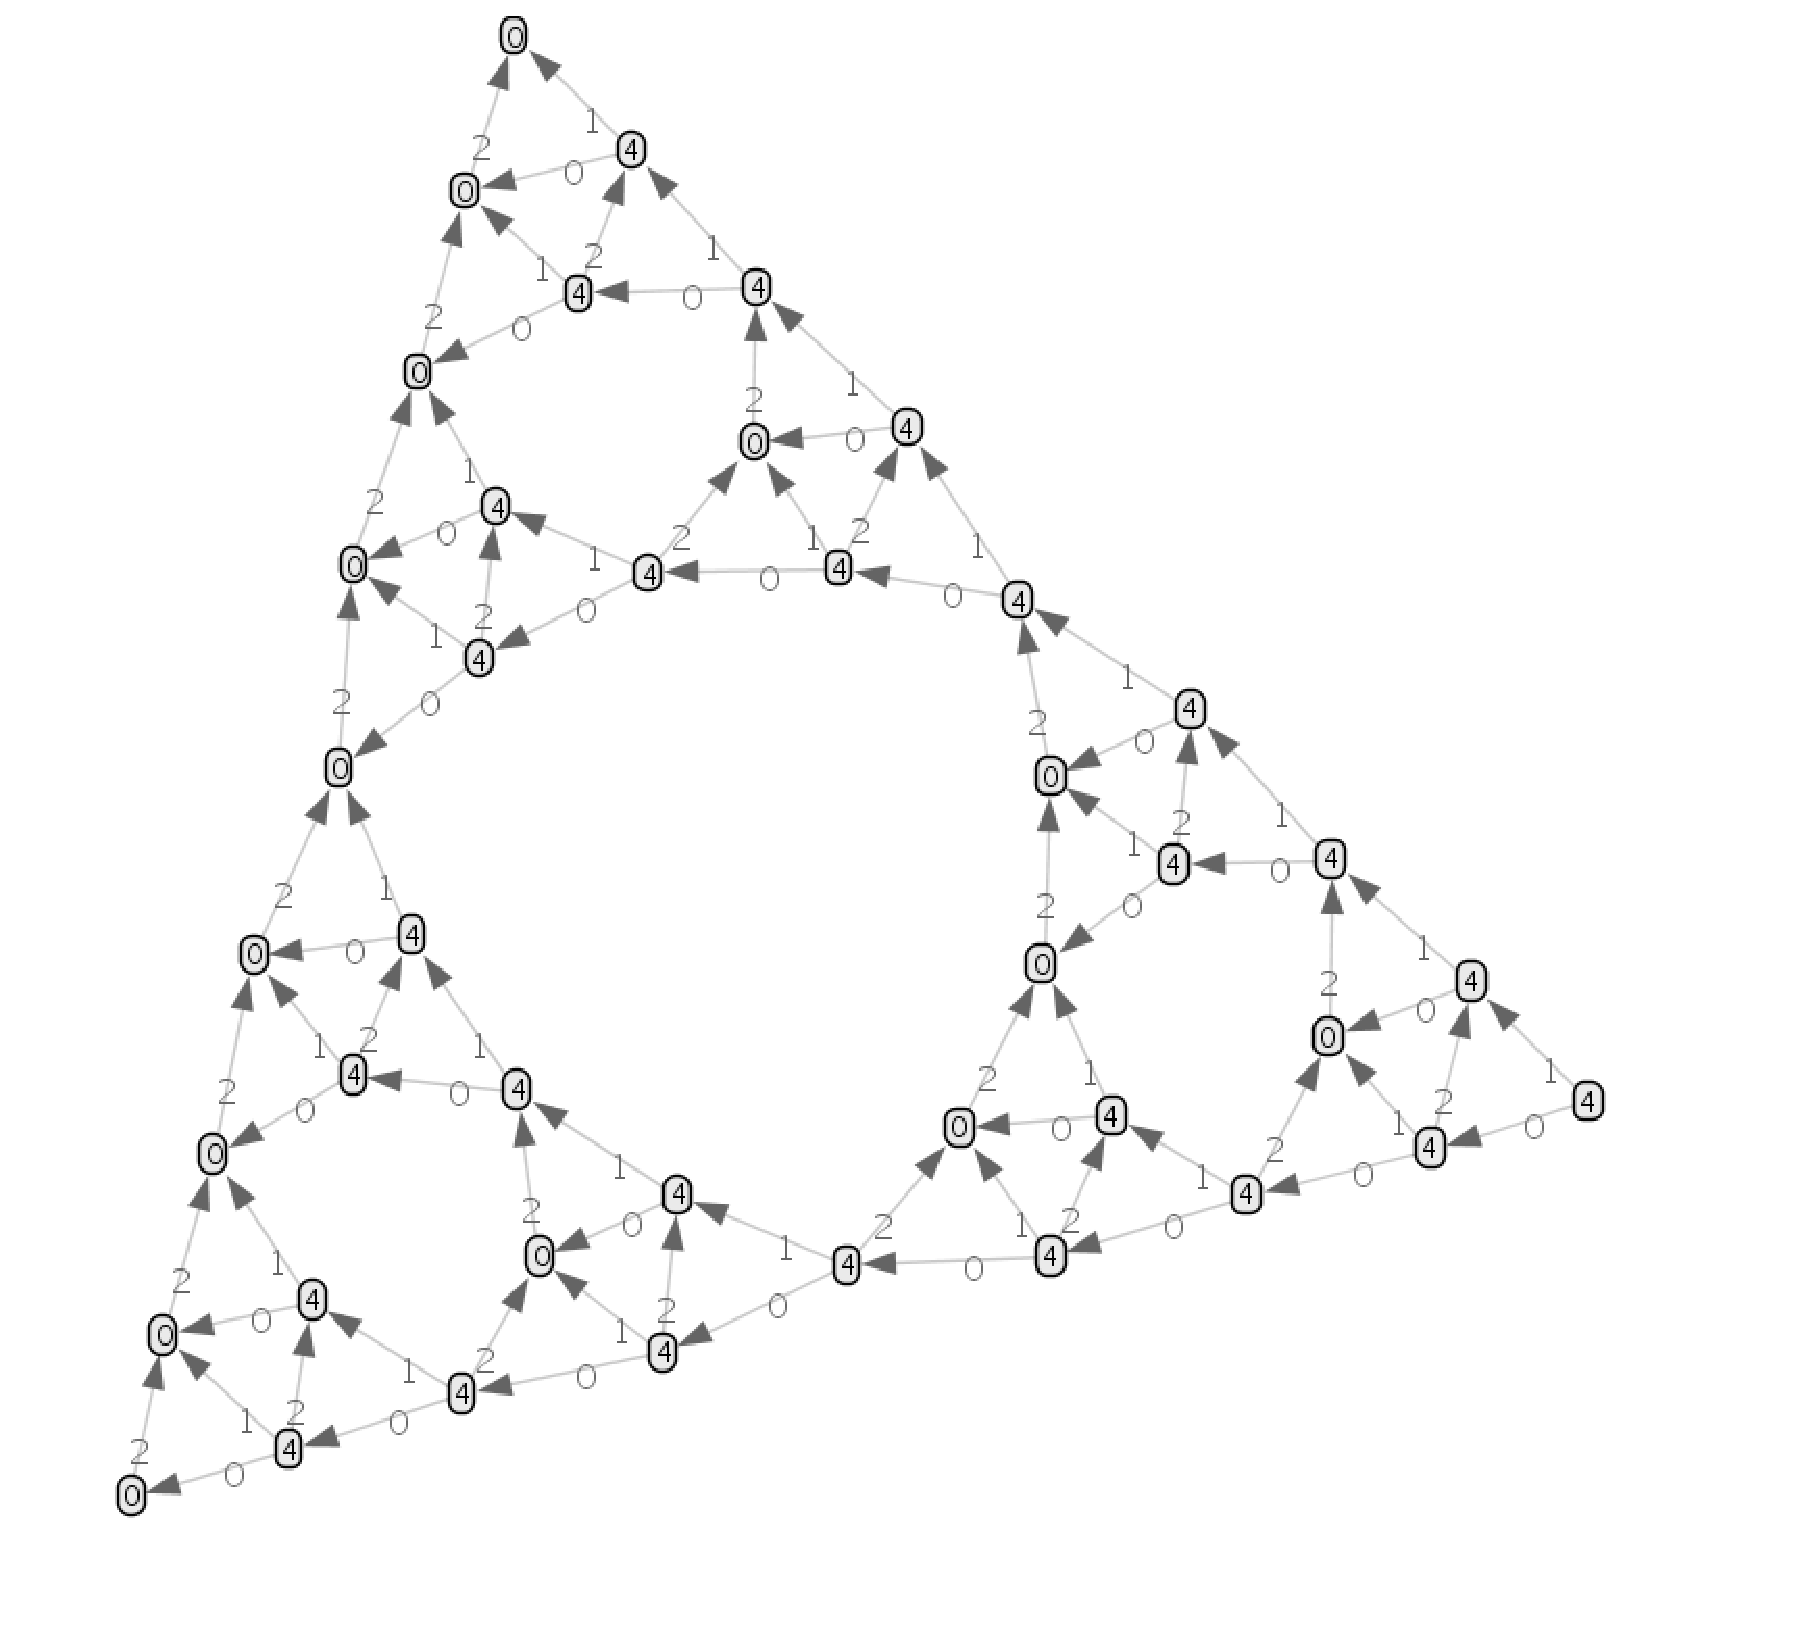
\includegraphics[scale=.35,angle=-15]{sierpinski-3.eps}
 \end{center}
\vspace*{-2.5cm}
\caption{Third generation Sierpinski triangle \label{fig:sierpinski}}
\end{figure}

After initialisation, the nested loop $\mtt{(inc;\, expand!)!}$ is executed. In each iteration of the outer loop, \texttt{inc} increases the current generation number if it is smaller than the required number (which is checked by the rule's condition). If the test is successful, the inner loop \ttt{expand!} performs a Sierpinski step on each triangle whose top node is labelled with the current generation number: the triangle is replaced by four triangles such that the top nodes of the three outer triangles are labelled with the next higher generation number. The test $\mathtt{x > y}$ fails when the required generation number has been reached. In this case the application of \texttt{inc} fails, causing the outer loop to terminate and return the current graph which is the Sierpinski triangle of the requested generation.

Sierpinski triangles pose a hard challenge for graph transformation: generating the $n$-th triangle requires space and a number of rule applications exponential in $n$. This problem was part of the 2007 tool contest for graph transformation, where the goal was to generate triangles of generation numbers as high as possible and as fast as possible \cite{Taentzer_et_al08a}.
